\documentclass{standalone}
\usepackage{tikz}
\begin{document}
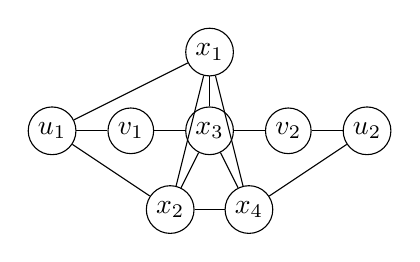
\begin{tikzpicture}[every node/.style={circle, draw, inner sep=2pt}]
  % P5 path (u1 - v1 - x3 - v2 - u2)
  \node (u1) at (0,0) {$u_1$};
  \node (v1) at (1,0) {$v_1$};
  \node (x3) at (2,0) {$x_3$};
  \node (v2) at (3,0) {$v_2$};
  \node (u2) at (4,0) {$u_2$};
  
  % Additional nodes connected to x3
  \node (x1) at (2,1)  {$x_1$};
  \node (x2) at (1.5,-1) {$x_2$};
  \node (x4) at (2.5,-1) {$x_4$};

  % Edges of the P5 path
  \draw (u1) -- (v1) -- (x3) -- (v2) -- (u2);
  
  % Connections from x3 to other nodes
  \draw (x3) -- (x1);
  \draw (x3) -- (x2);
  \draw (x3) -- (x4);
  
  % Triangle structure among x1, x2, x4
  \draw (x1) -- (x2);
  \draw (x1) -- (x4);
  \draw (x2) -- (x4);
  
  % Connections from u1/u2 to peripheral nodes
  \draw (u1) -- (x1);
  \draw (u1) -- (x2);
  \draw (u2) -- (x4);
\end{tikzpicture}
\end{document}